\documentclass[10pt,ngerman,aspectratio=169]{beamer}
\usepackage{lmodern}
\usepackage{amssymb,amsmath}
\usepackage{ifxetex,ifluatex}

\ifnum 0\ifxetex 1\fi\ifluatex 1\fi=0 % if pdftex
  \usepackage[T1]{fontenc}
  \usepackage[utf8]{inputenc}
\else % if luatex or xelatex
  \ifxetex
    \usepackage{mathspec}
  \else
    \usepackage{fontspec}
  \fi
  \defaultfontfeatures{Ligatures=TeX,Scale=MatchLowercase}
\fi
% use upquote if available, for straight quotes in verbatim environments
\IfFileExists{upquote.sty}{\usepackage{upquote}}{}
% use microtype if available
\IfFileExists{microtype.sty}{%
\usepackage{microtype}
\UseMicrotypeSet[protrusion]{basicmath} % disable protrusion for tt fonts
}{}
\usepackage{hyperref}
\PassOptionsToPackage{usenames,dvipsnames}{color} % color is loaded by hyperref
\hypersetup{unicode=true,
            pdftitle={Induktive Statistik},
            pdfauthor={Prof.~Dr.~Christoph Hanck},
            colorlinks=true,
            linkcolor=dueblue,
            citecolor=dueblue,
            urlcolor=dueblue,
            breaklinks=true}
\urlstyle{same}  % don't use monospace font for urls
\ifnum 0\ifxetex 1\fi\ifluatex 1\fi=0 % if pdftex
  \usepackage[shorthands=off,main=ngerman]{babel}
\else
  \usepackage{polyglossia}
  \setmainlanguage[]{}
\fi


\usepackage{color}
\usepackage{fancyvrb}
\newcommand{\VerbBar}{|}
\newcommand{\VERB}{\Verb[commandchars=\\\{\}]}
\DefineVerbatimEnvironment{Highlighting}{Verbatim}{commandchars=\\\{\}}
% Add ',fontsize=\small' for more characters per line
\usepackage{framed}
\definecolor{shadecolor}{RGB}{248,248,248}
\newenvironment{Shaded}{\begin{snugshade}}{\end{snugshade}}
\newcommand{\AlertTok}[1]{\textcolor[rgb]{0.94,0.16,0.16}{#1}}
\newcommand{\AnnotationTok}[1]{\textcolor[rgb]{0.56,0.35,0.01}{\textbf{\textit{#1}}}}
\newcommand{\AttributeTok}[1]{\textcolor[rgb]{0.13,0.29,0.53}{#1}}
\newcommand{\BaseNTok}[1]{\textcolor[rgb]{0.00,0.00,0.81}{#1}}
\newcommand{\BuiltInTok}[1]{#1}
\newcommand{\CharTok}[1]{\textcolor[rgb]{0.31,0.60,0.02}{#1}}
\newcommand{\CommentTok}[1]{\textcolor[rgb]{0.56,0.35,0.01}{\textit{#1}}}
\newcommand{\CommentVarTok}[1]{\textcolor[rgb]{0.56,0.35,0.01}{\textbf{\textit{#1}}}}
\newcommand{\ConstantTok}[1]{\textcolor[rgb]{0.56,0.35,0.01}{#1}}
\newcommand{\ControlFlowTok}[1]{\textcolor[rgb]{0.13,0.29,0.53}{\textbf{#1}}}
\newcommand{\DataTypeTok}[1]{\textcolor[rgb]{0.13,0.29,0.53}{#1}}
\newcommand{\DecValTok}[1]{\textcolor[rgb]{0.00,0.00,0.81}{#1}}
\newcommand{\DocumentationTok}[1]{\textcolor[rgb]{0.56,0.35,0.01}{\textbf{\textit{#1}}}}
\newcommand{\ErrorTok}[1]{\textcolor[rgb]{0.64,0.00,0.00}{\textbf{#1}}}
\newcommand{\ExtensionTok}[1]{#1}
\newcommand{\FloatTok}[1]{\textcolor[rgb]{0.00,0.00,0.81}{#1}}
\newcommand{\FunctionTok}[1]{\textcolor[rgb]{0.13,0.29,0.53}{\textbf{#1}}}
\newcommand{\ImportTok}[1]{#1}
\newcommand{\InformationTok}[1]{\textcolor[rgb]{0.56,0.35,0.01}{\textbf{\textit{#1}}}}
\newcommand{\KeywordTok}[1]{\textcolor[rgb]{0.13,0.29,0.53}{\textbf{#1}}}
\newcommand{\NormalTok}[1]{#1}
\newcommand{\OperatorTok}[1]{\textcolor[rgb]{0.81,0.36,0.00}{\textbf{#1}}}
\newcommand{\OtherTok}[1]{\textcolor[rgb]{0.56,0.35,0.01}{#1}}
\newcommand{\PreprocessorTok}[1]{\textcolor[rgb]{0.56,0.35,0.01}{\textit{#1}}}
\newcommand{\RegionMarkerTok}[1]{#1}
\newcommand{\SpecialCharTok}[1]{\textcolor[rgb]{0.81,0.36,0.00}{\textbf{#1}}}
\newcommand{\SpecialStringTok}[1]{\textcolor[rgb]{0.31,0.60,0.02}{#1}}
\newcommand{\StringTok}[1]{\textcolor[rgb]{0.31,0.60,0.02}{#1}}
\newcommand{\VariableTok}[1]{\textcolor[rgb]{0.00,0.00,0.00}{#1}}
\newcommand{\VerbatimStringTok}[1]{\textcolor[rgb]{0.31,0.60,0.02}{#1}}
\newcommand{\WarningTok}[1]{\textcolor[rgb]{0.56,0.35,0.01}{\textbf{\textit{#1}}}}
\usepackage{longtable,booktabs}
\IfFileExists{parskip.sty}{%
\usepackage{parskip}
}{% else
\setlength{\parindent}{0pt}
\setlength{\parskip}{3em plus 1pt minus 1pt}%{6pt plus 2pt minus 1pt}
}
\setlength{\emergencystretch}{3em}  % prevent overfull lines

\setcounter{secnumdepth}{0}
% Redefines (sub)paragraphs to behave more like sections
\ifx\paragraph\undefined\else
\let\oldparagraph\paragraph
\renewcommand{\paragraph}[1]{\oldparagraph{#1}\mbox{}}
\fi
\ifx\subparagraph\undefined\else
\let\oldsubparagraph\subparagraph
\renewcommand{\subparagraph}[1]{\oldsubparagraph{#1}\mbox{}}
\fi

%%% Use protect on footnotes to avoid problems with footnotes in titles
\let\rmarkdownfootnote\footnote%
\def\footnote{\protect\rmarkdownfootnote}


  \title{Induktive Statistik}
    \author{Prof.~Dr.~Christoph Hanck}
  
  \providecommand{\institute}[1]{}
  \expandafter\ifstrequal\expandafter{default}{default}{%
  \institute{\expandafter\ifstrequal\expandafter{de}{de}{%
  Universität Duisburg-Essen}{%
  University of Duisburg-Essen}}}{%
  
  \institute{default}
}


    \date{Sommersemester 2025}


% up until here https://github.com/rstudio/rmarkdown/blob/master/inst/rmd/latex/default-1.17.0.2.tex
%%%%%%%%%%%%%%%%%%%%%%%%%%%%%%%%%%%%%%%%%%%%%%%%%%%%%%%%%%%%%%%%%%%%%%%%%%%%%%%
%%% Additional packages
\makeatletter
\def\input@path{{"C:/Users/jens.klenke/AppData/Local/Programs/R/R-4.4.1/library/runidue/rmarkdown/templates/lectureslides/resources/"}}  % make them visible to tex to overcome warnings
\makeatother

%%This is style file ee.sty.
%%version 30/01/2002
%
\newcommand{\vnorm}[1]{\left|\!\left|#1\right|\!\right|}
%\newcommand{\lowexp}[1]{\raisebox{1.45mm}[-1.45mm]{\scriptsize{$#1$}}}
\newcommand{\lowexp}[2]{\raisebox{#2mm}[-#2mm]{\scriptsize{$#1$}}}
\newcommand{\newoperator}[3]{\newcommand*{#1}{\mathop{#2}#3}}
\newcommand{\renewoperator}[3]{\renewcommand*{#1}{\mathop{#2}#3}}
%
% symbols C,N,Q,R,Z for sets
\newcommand{\SC}{\mathbb{C}}
\newcommand{\SSS}{\mathbb{S}}
\newcommand{\SN}{\mathbb{N}}
\newcommand{\SQ}{\mathbb{Q}}
\newcommand{\SR}{\mathbb{R}}
\newcommand{\SZ}{\mathbb{Z}}
\newcommand{\SB}{\mathbb{B}}
%
% calligraphic capital letters
\newcommand{\calA}{\mathcal{A}}
\newcommand{\calB}{\mathcal{B}}
\newcommand{\calC}{\mathcal{C}}
\newcommand{\calD}{\mathcal{D}}
\newcommand{\calE}{\mathcal{E}}
\newcommand{\calF}{\mathcal{F}}
\newcommand{\calG}{\mathcal{G}}
\newcommand{\calH}{\mathcal{H}}
\newcommand{\calI}{\mathcal{I}}
\newcommand{\calJ}{\mathcal{J}}
\newcommand{\calK}{\mathcal{K}}
\newcommand{\calL}{\mathcal{L}}
\newcommand{\calM}{\mathcal{M}}
\newcommand{\calN}{\mathcal{N}}
\newcommand{\calO}{\mathcal{O}}
\newcommand{\calP}{\mathcal{P}}
\newcommand{\calQ}{\mathcal{Q}}
\newcommand{\calR}{\mathcal{R}}
\newcommand{\calS}{\mathcal{S}}
\newcommand{\calT}{\mathcal{T}}
\newcommand{\calU}{\mathcal{U}}
\newcommand{\calV}{\mathcal{V}}
\newcommand{\calW}{\mathcal{W}}
\newcommand{\calX}{\mathcal{X}}
\newcommand{\calY}{\mathcal{Y}}
\newcommand{\calZ}{\mathcal{Z}}
%
% bold lowercase and capital letters for vectors (v) and matrices (m)
\newcommand{\mA}{\bm A}
\newcommand{\va}{\bm a}
\newcommand{\mB}{\bm B}
\newcommand{\vb}{\bm b}
\newcommand{\mC}{\bm C}
\newcommand{\vc}{\bm c}
\newcommand{\mD}{\bm D}
\newcommand{\vd}{\bm d}
\newcommand{\mE}{\bm E}
\newcommand{\ve}{\bm e}
\newcommand{\mF}{\bm F}
\newcommand{\vf}{\bm f}
\newcommand{\mG}{\bm G}
\newcommand{\vg}{\bm g}
\newcommand{\mH}{\bm H}
\newcommand{\vh}{\bm h}
\newcommand{\mI}{\bm I}
\newcommand{\vi}{\bm i}
\newcommand{\mJ}{\bm J}
\newcommand{\vj}{\bm j}
\newcommand{\mK}{\bm K}
\newcommand{\vk}{\bm k}
\newcommand{\mL}{\bm L}
\newcommand{\vl}{\bm l}
\newcommand{\mM}{\bm M}
\newcommand{\vm}{\bm m}
\newcommand{\mN}{\bm N}
\newcommand{\vn}{\bm n}
\newcommand{\mO}{\bm O}
\newcommand{\vo}{\bm o}
\newcommand{\mP}{\bm P}
\newcommand{\vp}{\bm p}
\newcommand{\mQ}{\bm Q}
\newcommand{\vq}{\bm q}
\newcommand{\mR}{\bm R}
\newcommand{\vr}{\bm r}
\newcommand{\mS}{\bm S}
\newcommand{\vs}{\bm s}
\newcommand{\mT}{\bm T}
\newcommand{\vt}{\bm t}
\newcommand{\mU}{\bm U}
\newcommand{\vu}{\bm u}
\newcommand{\mV}{\bm V}
\newcommand{\vv}{\bm v}
\newcommand{\mW}{\bm W}
\newcommand{\vw}{\bm w}
\newcommand{\mX}{\bm X}
\newcommand{\vx}{\bm x}
\newcommand{\mY}{\bm Y}
\newcommand{\vy}{\bm y}
\newcommand{\mZ}{\bm Z}
\newcommand{\vz}{\bm z}
\newcommand{\vzero}{\bm 0}
\newcommand{\vone}{\bm 1}
%
% bold Greek lowercase letters for vectors (v)
\newcommand{\valpha}{\bm \alpha}
\newcommand{\vbeta}{\bm \beta}
\newcommand{\vgamma}{\bm \gamma}
\newcommand{\vdelta}{\bm \delta}
\newcommand{\vepsi}{\bm \epsi}
\newcommand{\vvarepsilon}{\bm \varepsilon}
\newcommand{\vzeta}{\bm \zeta}
\newcommand{\veta}{\bm \eta}
\newcommand{\vtheta}{\bm \theta}
\newcommand{\viota}{\bm \iota}
\newcommand{\vkappa}{\bm \kappa}
\newcommand{\vlambda}{\bm \lambda}
\newcommand{\vmu}{\bm \mu}
\newcommand{\vnu}{\bm \nu}
\newcommand{\vxi}{\bm \xi}
\newcommand{\vpi}{\bm \pi}
\newcommand{\vrho}{\bm \rho}
\newcommand{\vsigma}{\bm \sigma}
\newcommand{\vtau}{\bm \tau}
\newcommand{\vupsilon}{\bm \upsilon}
\newcommand{\vphi}{\bm \phi}
\newcommand{\vchi}{\bm \chi}
\newcommand{\vpsi}{\bm \psi}
\newcommand{\vomega}{\bm \omega}
%
% bold Greek capital letters for matrices (m)
\newcommand{\mGamma}{\bm \varGamma}
\newcommand{\mDelta}{\bm \varDelta}
\newcommand{\mTheta}{\bm \varTheta}
\newcommand{\mLambda}{\bm \varLambda}
\newcommand{\mXi}{\bm \varXi}
\newcommand{\mXib}{\bm \Xi}
\newcommand{\mPi}{\bm \varPi}
\newcommand{\mSigma}{\bm \varSigma}
\newcommand{\mUpsilon}{\bm \varUpsilon}
\newcommand{\mPhi}{\bm \varPhi}
\newcommand{\mPsi}{\bm \varPsi}
\newcommand{\mOmega}{\bm \varOmega}
%
% roman letters in mathematics
\newcommand{\rb}{\ensuremath{\mathrm{b}}}
\newcommand{\rB}{\ensuremath{\mathrm{B}}}
\newcommand{\rC}{\ensuremath{\mathrm{C}}}
\newcommand{\rD}{\ensuremath{\mathrm{D}}}
\newcommand{\rf}{\ensuremath{\mathrm{f}}}
\newcommand{\rF}{\ensuremath{\mathrm{F}}}
\newcommand{\rH}{\ensuremath{\mathrm{H}}}
\newcommand{\rL}{\ensuremath{\mathrm{L}}}
\newcommand{\rN}{\ensuremath{\mathrm{N}}}
\newcommand{\rt}{\ensuremath{\mathrm{t}}}
\newcommand{\rU}{\ensuremath{\mathrm{U}}}
\newcommand{\rGam}{\ensuremath{\mathrm{Gam}}}
\newcommand{\rBeta}{\ensuremath{\mathrm{Beta}}}
%
\newcommand{\Bin}{\ensuremath{\mathrm{Bin}}}
\newcommand{\eu}{\ensuremath{\mathrm{e}}}
\newcommand{\iu}{\ensuremath{\mathrm{i}}}
\newcommand{\LN}{\ensuremath{\mathrm{LN}}}
\newcommand{\IN}{\ensuremath{\mathrm{IN}}}

\newcommand{\Poi}{\ensuremath{\mathrm{Poi}}}
%
\newcommand{\ped}[1]{\ensuremath{_\mathrm{#1}}} %pedex
\newcommand{\ap}[1]{\ensuremath{^\mathrm{#1}}} %apex
\renewoperator{\Re}{\mathrm{Re}}{\nolimits}
\renewoperator{\Im}{\mathrm{Im}}{\nolimits}
%
% letters for (partial) differentiation
%\newcommand{\rd}{\ensuremath{\mathrm{d}}}
\makeatletter
\newcommand{\rd}{\@ifnextchar^{\DIfF}{\DIfF^{}}}
\def\DIfF^#1{%
   \mathop{\mathrm{\mathstrut d}}%
   \nolimits^{#1}\gobblespace}
\def\gobblespace{\futurelet\diffarg\opspace}
\def\opspace{%
   \let\DiffSpace\!%
   \ifx\diffarg(%
   \let\DiffSpace\relax
   \else
   \ifx\diffarg[%
   \let\DiffSpace\relax
   \else
   \ifx\diffarg\{%
   \let\DiffSpace\relax
   \fi\fi\fi\DiffSpace}
\newcommand{\deriv}[3][]{\frac{\rd^{#1}#2}{\rd #3^{#1}}}
\newcommand{\pderiv}[3][]{\frac{\partial^{#1}#2}{\partial #3^{#1}}}
%
% operatornames
\newcommand{\Avar}{\operatorname{Avar}}
\newcommand{\bias}{\operatorname{bias}}
\newcommand{\col}{\operatorname{col}}
\newcommand{\corr}{\operatorname{corr}}
\newcommand{\Corr}{\operatorname{Corr}}
\newcommand{\cov}{\operatorname{cov}}
\newcommand{\Cov}{\operatorname{Cov}}
\newcommand{\dg}{\operatorname{dg}}
\newcommand{\diag}{\operatorname{diag}}
\newcommand{\E}{\operatorname{E}}
\newcommand{\etr}{\operatorname{etr}}
\newoperator{\ip}{\mathrm{int}}{\nolimits}
\newcommand{\kur}{\operatorname{kur}}
%\newcommand{\median}{\operatorname{med}}
\newcommand{\MSE}{\operatorname{MSE}}
\newcommand{\plim}{\operatorname{plim}}
%\newcommand{\plim}{\DeclareMathOperator{plim}}
\newcommand{\cond}{\rightarrow_{\mathrm{d}}}
\newcommand{\conp}{\rightarrow_{\mathrm{p}}}
\newcommand{\rk}{\operatorname{rk}}
\newcommand{\sgn}{\operatorname{sgn}}
\newcommand{\spur}{\operatorname{spur}}
\newcommand{\tr}{\operatorname{tr}}
\newcommand{\var}{\operatorname{Var}}
\newcommand{\Var}{\operatorname{Var}}
\renewcommand{\vec}{\operatorname{vec}}
\newcommand{\vech}{\operatorname{vech}}
\DeclareMathOperator*{\argmin}{arg\,min}
\DeclareMathOperator*{\argmax}{arg\,max}
%
% other definitions
\newcommand{\distr}{\sim}
\newcommand{\adistr}{\stackrel{a}{\distr}}
\newcommand{\diff}{\Delta}
\newcommand{\fordiff}{\bigtriangleup}
\newcommand{\fdiff}{\diff_{\rf}}
\newcommand{\bdiff}{\diff_{\rb}}
%
%\mathchardef\varepsilon="010F
%\mathchardef\epsilon="0122
%\mathchardef\eps="010F
\newcommand{\eps}{\epsilon}
\newcommand{\epsi}{\varepsilon}
%
\newcommand{\longto}{\longrightarrow}
\newcommand{\pto}{\stackrel{p}{\longrightarrow}}
\newcommand{\dto}{\stackrel{d}{\longrightarrow}}
\newcommand{\wto}{\stackrel{w}{\longrightarrow}}
%
\newcommand{\Infmat}{\bm\calI}
\newcommand{\Hesmat}{\bm\calH}
\newcommand{\bcdot}{\raisebox{1pt}{\textbf{\large .}}}
\newcommand{\interior}[1]{\overset{\circ}{#1}}
%
\newcommand{\vones}{\bm\imath}
\newcommand{\vzeros}{\boldsymbol{0}}
\newcommand{\mZeros}{\mathbf{O}}
%
% additional commands
\newcommand{\EE}[1]{\E\left(#1\right)}
\renewcommand{\Pr}{\ensuremath{\mathrm{P}}}
\newcommand{\prob}[1]{\Pr\left(#1\right)}
\newcommand{\Prob}[1]{\Pr\left(#1\right)}
\newcommand{\Spur}[1]{\spur\left[#1\right]}
\newcommand{\vvarphi}{\bm \varphi}
%

\usepackage{BeamerColor}
\usepackage{hypernat}
\usepackage{mathtools}
\usepackage[export]{adjustbox}
\usepackage{makecell}
\usepackage{diagbox}
\usepackage{bm, bbm}
\usepackage{subfig}
\usepackage{forest}
\usepackage[labelfont={footnotesize,color=dueblue},font=footnotesize]{caption}
\usepackage{soul}
\usepackage{textcomp}
\usepackage{zref}
\usepackage{zref-user}
\usepackage{zref-xr}
\usepackage{empheq}
\usepackage{tikz}
\usetikzlibrary{arrows, decorations.markings}
\tikzstyle{arrow} = [ultra thick, - latex, shorten >= 2pt, shorten <= 2pt] % default arrow
\tikzstyle{vecArrow} = [thick, decoration={markings,mark=at position
	1 with {\arrow[semithick]{open triangle 60}}},
double distance=1.4pt, shorten >= 5.5pt,
preaction = {decorate},
postaction = {draw,line width=1.4pt, white,shorten >= 4.5pt}]
\tikzstyle{innerWhite} = [semithick, white,line width=1.4pt, shorten >= 4.5pt] % vec arrow
\tikzstyle{box} = [rectangle,rounded corners,fill=dueblue, text=white, align=center, node distance=1.25cm] % default node

% \usepackage{etoolbox}

\makeatletter
\let\@@magyar@captionfix\relax
\makeatother

%%% ZREF

%%% New colors
\definecolor{dueblue}{RGB}{0,76,147}
\definecolor{duelightblue}{RGB}{223,228,242}
\definecolor{duebeige}{RGB}{239,228,191}
\definecolor{darkgrey}{RGB}{40, 40, 40}
\definecolor{salmon}{RGB}{239, 148, 108}
\definecolor{lime}{RGB}{219, 254, 135}
\definecolor{sandy}{RGB}{255, 227, 129}
\definecolor{darklime}{RGB}{153, 194, 77}


%%% Additional commands
\newcommand{\npt}{\\[1ex]\pause}
\newcommand{\nbs}{\protect{~}}
\newcommand{\qedb}{\hfill \textsquare} % to be used outside proof environments
\newcommand{\pausealt}{ }
\newcommand{\blue}[1]{{\color{dueblue}{#1}\color{black}}}
\newcommand{\hil}[1]{\textbf{\color{dueblue}{#1}\color{black}}}
\newcommand{\hilm}[1]{\mathbf{\color{dueblue}{#1}\color{black}}}
\newcommand{\mps}{\par\medbreak}
\newcommand{\sd}{\operatorname{sd}}
\newcommand{\SD}{\operatorname{SD}}

% Kahoot Block
\newenvironment<>{kahoot}[1]{%
  \begin{actionenv}#2%
      \def\insertblocktitle{#1}%
      \par%
      \mode<presentation>{%
      \setbeamercolor{block title}{fg=black,bg=yellow}
       \setbeamercolor{block body}{fg=black,bg=yellow!20}
       \setbeamercolor{itemize item}{fg=orange!20!black}
       \setbeamertemplate{itemize item}[triangle]
     }%
      \usebeamertemplate{block begin}
      \begin{center}
\includegraphics[width=0.25\textwidth]{"C:/Users/jens.klenke/AppData/Local/Programs/R/R-4.4.1/library/runidue/rmarkdown/templates/lectureslides/resources/kahootlogo2"}
\end{center}}
    {\par\usebeamertemplate{block end}\end{actionenv}}
\newcommand{\kahootblock}[1]{\begin{kahoot}{#1}\end{kahoot}}

% QuizAcademy Block
\newenvironment<>{QuizAcademy}[1]{%
	\begin{actionenv}#2%
		\def\insertblocktitle{#1}%
		\par%
		\mode<presentation>{%
			\setbeamercolor{block title}{fg=black,bg=yellow}
			\setbeamercolor{block body}{fg=black,bg=yellow!20}
			\setbeamercolor{itemize item}{fg=orange!20!black}
			\setbeamertemplate{itemize item}[triangle]
		}%
		\usebeamertemplate{block begin}
		\begin{center}
			\includegraphics[width=0.25\textwidth]{"C:/Users/jens.klenke/AppData/Local/Programs/R/R-4.4.1/library/runidue/rmarkdown/templates/lectureslides/resources/QuizAcademy.png"}
	\end{center}}
	{\par\usebeamertemplate{block end}\end{actionenv}}
\newcommand{\QuizAcademyblock}[1]{\begin{QuizAcademy}{#1}\end{QuizAcademy}}



% Rlogo
\makeatletter
\newcommand*\fsize{\dimexpr\f@size pt\relax} % returns current font size
\makeatother
\newcommand{\R}{\includegraphics[height=.85\fsize, clip=T]{"C:/Users/jens.klenke/AppData/Local/Programs/R/R-4.4.1/library/runidue/rmarkdown/templates/lectureslides/resources/Rlogo"}\ }
\newcommand{\btVFill}{\vskip0pt plus 1filll}
\newcommand{\source}[1]{\btVFill\scriptsize \textit{\expandafter\ifstrequal\expandafter{de}{de}{Quelle: }{Source: }}#1}



% BLOCK ENVIRONMENTS (THEOREMS)
\expandafter\ifstrequal\expandafter{box}{blank}{
}{
\setbeamerfont{block title}{size=\normalsize}
\setbeamercolor{block title}{bg=duelightblue,fg=black}
\setbeamercolor{block body}{bg=duelightblue!37,fg=black}
}%
\setbeamertemplate{blocks}[rounded][shadow=false]

% Headers for theorems
\expandafter\ifstrequal\expandafter{de}{de}{%
  \newcommand{\thmncont}{Fortsetzung}
  \newtheorem{thmn}{Theorem}[section]
  \newtheorem{lem}[thmn]{Lemma}
  \newtheorem{cor}[thmn]{Corollary}
  \newtheorem{defn}[thmn]{Definition}
  \newtheorem{ass}[thmn]{Annahme}
  \newtheorem{rem}[thmn]{Anmerkung}
  \newtheorem{prop}[thmn]{Proposition}
  \theoremstyle{definition}
  \newtheorem{xmpl}[thmn]{Beispiel}
  \newtheorem{que}[thmn]{Frage}
  \newtheorem{exe}[thmn]{Aufgabe}
  \numberwithin{equation}{section}}{%%%
  \newcommand{\thmncont}{Continued}
  \newtheorem{thmn}{Theorem}[section]
  \newtheorem{lem}[thmn]{Lemma}
  \newtheorem{cor}[thmn]{Corollary}
  \newtheorem{defn}[thmn]{Definition}
  \newtheorem{ass}[thmn]{Assumption}
  \newtheorem{rem}[thmn]{Remark}
  \newtheorem{prop}[thmn]{Proposition}
  \theoremstyle{definition}
  \newtheorem{xmpl}[thmn]{Example}
  \newtheorem{que}[thmn]{Question}
  \newtheorem{exe}[thmn]{Exercise}
  \numberwithin{equation}{section}
}%

% CONTINUING BLOCKS
\newenvironment{thmn*}{\addtocounter{thmn}{-1}\thmn[\thmncont]}{\endthmn}
\newenvironment{lem*}{\addtocounter{thmn}{-1}\lem[\thmncont]}{\endlem}
\newenvironment{cor*}{\addtocounter{thmn}{-1}\cor[\thmncont]}{\endcor}
\newenvironment{defn*}{\addtocounter{thmn}{-1}\thmn[\thmncont]}{\endthmn}
\newenvironment{ass*}{\addtocounter{thmn}{-1}\ass[\thmncont]}{\endass}
\newenvironment{rem*}{\addtocounter{thmn}{-1}\rem[\thmncont]}{\endrem}
\newenvironment{xmpl*}{\addtocounter{thmn}{-1}\xmpl[\thmncont]}{\endxmpl}
\newenvironment{que*}{\addtocounter{thmn}{-1}\que[\thmncont]}{\endque}


\setbeamertemplate{theorems}[numbered]
\setbeamerfont{block title}{size=\normalsize}
\setbeamertemplate{theorem begin}
{%
  \expandafter\ifstrequal\expandafter{\inserttheoremaddition}{*}{\addtocounter{thmn}{-1}}{}
  \normalfont
  \begin{\inserttheoremblockenv}{%
    \structure{%
      \textcolor{darkgrey}{\textbf{\inserttheoremname \inserttheoremnumber}:
      \ifx\inserttheoremaddition\empty\else\expandafter\ifstrequal\expandafter{\inserttheoremaddition}{*}{\thmncont\inserttheorempunctuation}{\inserttheoremaddition\inserttheorempunctuation}\fi}%
    }%
  }%
}
\setbeamertemplate{theorem end}{\leavevmode\end{\inserttheoremblockenv}}

\preto{\xmpl}{
    \setbeamercolor{block title}{fg=black,bg=sandy!70!white}
    \setbeamercolor{block body}{fg=black, bg=sandy!20!white}
}

\preto{\exe}{
    \setbeamercolor{block title}{fg=black,bg=darklime!70!white}
    \setbeamercolor{block body}{fg=black, bg=darklime!20!white}
}




% Spacings
\AtBeginEnvironment{figure}{\setlength{\parskip}{-2ex}}
\AtBeginEnvironment{center}{\smallbreak}
\AtEndEnvironment{center}{\smallbreak}
\AtBeginEnvironment{itemize}{\smallskip \setlength{\itemsep}{0.3ex}\setlength{\parskip}{1ex}}
\AtEndEnvironment{itemize}{\smallskip}
\preto{\enumerate}{\medskip  \setlength{\itemsep}{0.75ex}\setlength{\parskip}{1ex}}
\AtEndEnvironment{enumerate}{\smallskip}



% \let\tempone\itemize
% \let\temptwo\enditemize
% \renewenvironment{itemize}{\tempone\setlength{\itemsep}{1ex}\setlength{\parskip}{1.2ex}}{\temptwo}

% \let\tempone\enumerate
% \let\temptwo\endenumerate
% \renewenvironment{enumerate}{\tempone\setlength{\itemsep}{1ex}\setlength{\parskip}{1.2ex}}{\temptwo}
% 




%%% LAYOUT
\usecolortheme[named=dueblue]{structure}
\beamertemplatenavigationsymbolsempty
\setbeamersize{text margin left=10pt, text margin right=10pt}


% Spacing before and after code chunks / output
\makeatletter
\preto{\@verbatim}{\topsep=-2pt \partopsep=2pt \parskip=-2ex}
\makeatother

% spacing before figure captions
\setlength{\abovecaptionskip}{0pt}
\setlength{\belowcaptionskip}{-1em plus 1em minus 0em}

% spacing aorund display equations
\setlength{\abovedisplayskip}{3pt}
%\setlength{\belowdisplayskip}{3pt}

 % 

% Frame Head
\makeatletter
\setbeamertemplate{frametitle}{%
\vspace{.1cm}
\begin{minipage}[t][1cm]{1\textwidth}
    \ifbeamer@plainframe%
      \Large\insertframetitle%
    \else
      \Large\insertframetitle%
      \hfill
      \includegraphics[width=2cm,keepaspectratio=true, valign=t]{"C:/Users/jens.klenke/AppData/Local/Programs/R/R-4.4.1/library/runidue/rmarkdown/templates/lectureslides/resources/duelogo"} 
      \ifx\insertframesubtitle\empty
      \else
        \\ \small \insertframesubtitle
      \fi
    \fi
\end{minipage}

}
\makeatother

%%\includegraphics[width=2cm,keepaspectratio=true, valign=t]{"C:/Users/jens.klenke/AppData/Local/Programs/R/R-4.4.1/library/runidue/rmarkdown/templates/lectureslides/resources/duelogo"}
%    





% Footer
\setbeamercolor{footlinecolor}{bg=dueblue,fg=white}


\ifstrequal{default}{colored}{
\setbeamertemplate{footline}{
  % \hbox{
  \begin{beamercolorbox}[wd=\paperwidth,ht=0.4cm, leftskip=0cm, rightskip=0cm]{footlinecolor}
    \hfill \scriptsize{{\insertshortauthor : }
    \insertshorttitle---\insertsection \hfill \thesection-\insertframenumber\hspace*{.15cm}}\vspace{1mm}
  \end{beamercolorbox}
  % }
}
\addtobeamertemplate{footline}{\hypersetup{linkcolor=.}}{}
}{
\setbeamertemplate{footline}{\hspace*{.1cm}%
\hfill \scriptsize{{\insertshortauthor : }
\insertshorttitle---\insertsection \hfill \thesection-\insertframenumber\hspace*{.2cm}}\vspace{1mm}}
}




% TOC


\setbeamertemplate{section in toc shaded}[default][50]
\defbeamertemplate{section in toc}{customcircle}
{\leavevmode\leftskip=4ex%
  \llap{%
    \usebeamerfont*{section number projected}%
    \usebeamercolor{section number projected}%
    \begin{pgfpicture}{-1ex}{-.2ex}{1ex}{2ex}
      \color{bg}
      \pgfpathcircle{\pgfpoint{0pt}{.75ex}}{1.3ex}
      \pgfusepath{fill}
      \pgftext[base]{\color{fg}\inserttocsectionnumber}
    \end{pgfpicture}\kern1.25ex%
  }%
  \hspace{0.8ex}\inserttocsection\par}

\setbeamertemplate{section in toc}[customcircle]

% \usepackage{xpatch}
% \xpatchcmd{\itemize}
%   {\def\makelabel}
%   {\setlength{\itemsep}{1ex}\def\makelabel}
%   {}
%   {}
% \makeatletter
% \xpatchcmd{\beamer@enum@}
%   {\def\makelabel}
%   {\setlength{\itemsep}{1ex}\def\makelabel}
%   {}
%   {}
% \makeatother

% NEW SECTION


\AtBeginSection[] {
{
\setbeamertemplate{footline}{}
\begin{frame}{\expandafter\ifstrequal\expandafter{de}{de}{Überblick}{Outline}}
\vspace{0.5cm}
\tableofcontents[currentsection]
\end{frame}
\addtocounter{framenumber}{-\insertframenumber} % collect all begin section commands in one env.!
}
}

% ITEMIZE, ENUMERATE, DESCRIPTION
\defbeamertemplate*{description item}{defaultperiod}{\insertdescriptionitem.}
\setbeamersize{description width=15pt} % left margin for description

\setlength{\topsep}{1ex}
\setlength{\leftmargini}{10pt+.5\labelwidth}
\setlength{\leftmarginii}{15pt}
\setlength{\leftmarginiii}{15pt}


\setbeamertemplate{caption}[numbered]
\setbeamertemplate{caption label separator}{: }
\setbeamertemplate{itemize item}[circle]
\setbeamertemplate{itemize subitem}[triangle]
\setbeamertemplate{enumerate item}[default]
\setbeamertemplate{enumerate subitem}[default]
\setbeamertemplate{description item}[defaultperiod]
\setbeamertemplate{description subitem}[defaultperiod]


\providecommand{\tightlist}{}% \setlength{\itemsep}{0.75ex}\setlength{\parskip}{1.2ex}
% allow environments inside environments
\let\otherbegin\begin
\let\otherend\end
%%%%%%%%%%%%%%%%%%%%%%%%%%%%%%%%%%%%%%%%%%%%%%%%%%%%%%%%%%%%%%%%%%%%%%%%%%%%%%%
% from here on https://github.com/rstudio/rmarkdown/blob/master/inst/rmd/latex/default-1.17.0.2.tex



\begin{document}


      {\usebackgroundtemplate{\includegraphics[scale=0.25]{"C:/Users/jens.klenke/AppData/Local/Programs/R/R-4.4.1/library/runidue/rmarkdown/templates/lectureslides/resources/duetower"}}
    \frame[plain]{\titlepage}}
  

% 
\section{Einleitung}\label{einleitung}

\begin{frame}{Motivation}
\phantomsection\label{motivation}
\begin{itemize}
\tightlist
\item
  Ziel der \hil{deskriptiven} (beschreibenden) \hil{Statistik}: das
  Datenmaterial mit Hilfe tabellarischer und grafischer Repräsentationen
  sowie geeigneter Kenngrößen übersichtlich aufbereiten.
\item
  Ziel der \hil{induktiven} (schließenden) \hil{Statistik}: Verifikation
  theoretischer Modelle anhand von Daten und Testen von Hypothesen über
  unbekannte Parameter auf Basis von Wahrscheinlichkeitsmodellen.
\end{itemize}
\end{frame}

\begin{frame}{Motivation}
\phantomsection\label{motivation-1}
\framesubtitle{Beispiel: Lernerfolg}

\footnotesize
\begin{center}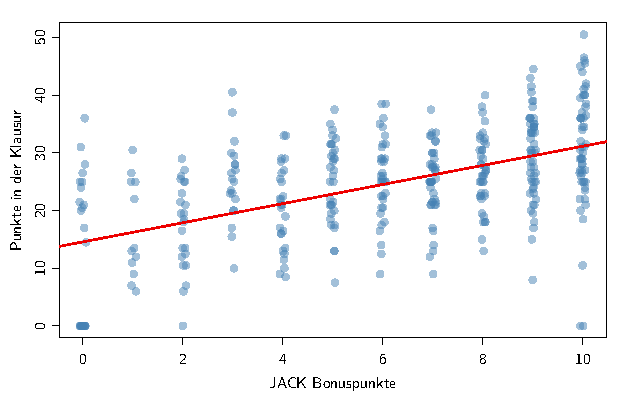
\includegraphics{Resources/Plots/unnamed-chunk-2-1} \end{center}
\normalsize
\end{frame}

\begin{frame}{Motivation}
\phantomsection\label{motivation-2}
Übergang von der deskriptiven zur induktiven Statistik:

\begin{itemize}
\tightlist
\item
  \hil{Induktives Schließen}, statistische Inferenz,
  Repräsentationsschluss: Schluss von einer Teilgesamtheit auf die
  Grundgesamtheit
\item
  \hil{Induktive Statistik}: Methoden, die es erlauben von den
  Beobachtungen einer Teilgesamtheit \linebreak (= \emph{Stichprobe})
  auf bestimmte Charakteristika der dazugehörenden
  \emph{Grundgesamtheit} zu schließen.
\end{itemize}
\end{frame}

\begin{frame}{Motivation}
\phantomsection\label{motivation-3}
\begin{itemize}
\tightlist
\item
  Beim Glücksspiel meinen Sie, dass die \glqq{}Gegenseite\grqq{} mit
  manipulierten Würfeln spielt, d.h. die Zahl 6 fällt häufiger als
  andere Zahlen. Wie können Sie Ihre Vermutung überprüfen?
\item
  Vor der Bundestagswahl prognostiziert ein Wahlforschungsinstitut, dass
  30\% der Stimmen auf die CDU/CSU entfallen. Wie kann eine solche
  Prognose verlässlich durchgeführt werden?
\end{itemize}

Ziel: Schlussfolgerungen von einer Stichprobe auf die Grundgesamtheit
\end{frame}

\begin{frame}{Motivation}
\phantomsection\label{motivation-4}
\framesubtitle{QuizAcademy}

\QuizAcademy{Schokoladenwürfel}\endQuizAcademy
\end{frame}

\begin{frame}{Motivation}
\phantomsection\label{motivation-5}
\begin{center}
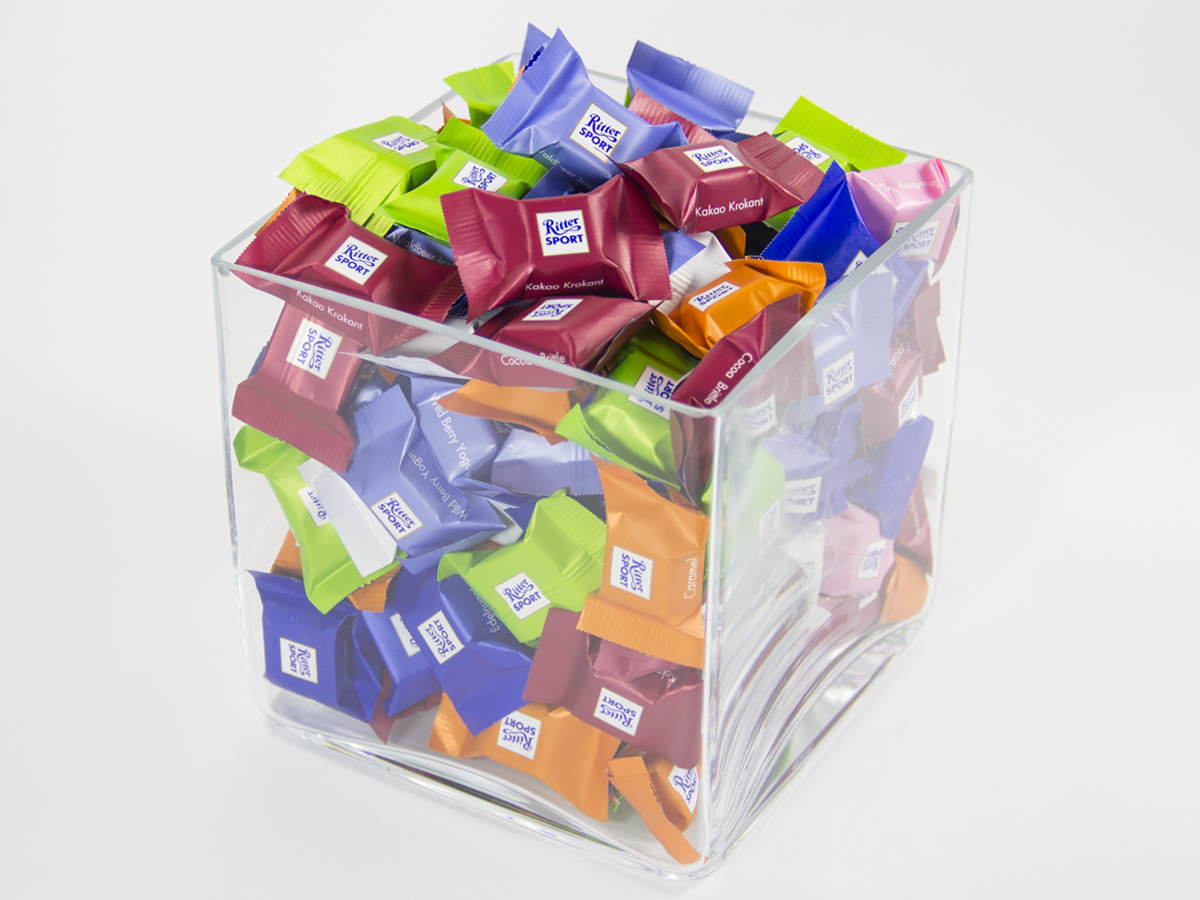
\includegraphics[height=0.6\textheight, keepaspectratio]{Resources/Grafiken/Schaetzen.jpg}
\end{center}
\source{\href{https://blog.ritter-sport.de/2014/08/05/schatzt-euch-bunt/}{https://blog.ritter-sport.de/2014/08/05/schatzt-euch-bunt/}}
\end{frame}

\begin{frame}{Motivation}
\phantomsection\label{motivation-6}
Man beachte: Wahrscheinlichkeitsrechnung

\begin{itemize}
\tightlist
\item
  ist \textbf{mehr} als Grundlage der schließenden Statistik
\item
  hat enorme eigenständige ökonomische Bedeutung z.B. in der

  \begin{itemize}
  \tightlist
  \item
    Mikroökonomik
  \item
    Investition und Finanzierung
  \item
    Portfoliotheorie
  \end{itemize}
\end{itemize}
\end{frame}

\begin{frame}{Gliederung}
\phantomsection\label{gliederung}
\begin{enumerate}
\tightlist
\item
  Einleitung
\item
  Grundlagen
\item
  Eindimensionale Zufallsvariablen
\item
  Ausgewählte theoretische Verteilungen
\item
  Grundzüge der Stichprobentheorie
\item
  Statistische Schätzverfahren
\item
  Statistische Testverfahren
\item
  Zweidimensionale Zufallsvariablen
\end{enumerate}
\end{frame}

\section{Grundlagen}\label{grundlagen}

\begin{frame}{Grundlegende Begriffe}
\phantomsection\label{grundlegende-begriffe}
\framesubtitle{Zufallsvorgang}

Zufallsvorgänge (bzw. stochastische Vorgänge) sind durch zwei
wesentliche Eigenschaften gekennzeichnet:

\begin{enumerate}
\tightlist
\item
  Sie besitzen verschiedene, sich gegenseitig ausschließende Ausgänge,
  die bereits vor Beginn des Vorgangs bekannt sind;
\item
  es ist nicht vorhersehbar, welcher Ausgang tatsächlich eintreten wird.
\end{enumerate}

\hil{Beispiele} für Zufallsvorgänge:

\begin{itemize}
\tightlist
\item
  Der Ausgang eines Fußballspiels, der Kurs einer Aktie am nächsten Tag
  oder die realisierte Augenzahl eines Würfelwurfes.
\end{itemize}
\end{frame}

\begin{frame}{Grundlegende Begriffe}
\phantomsection\label{grundlegende-begriffe-1}
\framesubtitle{Zufallsvorgang, Zufallsexperiment}

\begin{itemize}
\tightlist
\item
  Ist ein Zufallsvorgang unverändert beliebig oft wiederholbar, liegt
  ein \hil{Zufallsexperiment} vor. Die unveränderte Wiederholbarkeit
  beschreibt man auch als unter gleichen (Rand-)Bedingungen
  wiederholbar.
\item
  D.h., dass die Randbedingungen wie bei naturwissenschaftlichen
  Experimenten kontrolliert werden können. Dies stellt sicher, dass die
  Bedingungen, unter denen das Experiment stattgefunden hat, auch bei
  weiteren Durchführungen hätten eingehalten werden können.
\item
  Damit gehören alle Zufallsvorgänge, die fiktiv unter gleichen
  Bedingungen wiederholbar sind, zu den Zufallsexperimenten. Dies
  erlaubt es, auch Zufallsvorgänge als Zufallsexperimente aufzufassen,
  deren praktische Wiederholung unter gleichen Bedingungen schwierig
  wäre.
\end{itemize}
\end{frame}

\begin{frame}{Grundlegende Begriffe}
\phantomsection\label{grundlegende-begriffe-2}
\framesubtitle{Zufallsvorgang, Zufallsexperiment, Stichprobenraum}

\begin{itemize}
\tightlist
\item
  Alle Ausgänge \(\omega_i\) eines Zufallsvorganges bzw. -experimentes
  fasst man zu einem \hil{Stichprobenraum} (Ergebnis- bzw. Ereignisraum)
  \(\Omega\) zusammen. Der Stichprobenraum ist eine Menge, deren
  Elemente die Ausgänge sind.
\item
  \(\Omega\) kann endlich oder unendlich viele Ausgänge enthalten.
  Lassen sich die unendlich vielen Ausgänge mit den natürlichen Zahlen
  \(\mathbb{N}\) abzählen, bezeichnet man \(\Omega\) als
  \hil{abzählbar unendlich}. Gelingt dies nicht, heißt \(\Omega\)
  \hil{überabzählbar unendlich}.
\end{itemize}

\[\Omega=\{\omega_1,\ldots,\omega_m,\ldots\}.\]
\end{frame}

\begin{frame}{Grundlegende Begriffe}
\phantomsection\label{grundlegende-begriffe-3}
\framesubtitle{Zufallsvorgang, Zufallsexperiment, Stichprobenraum}

\xmpl[Würfelwurf]Der Zufallsvorgang \emph{Werfen eines Würfels} hat
sechs mögliche Ausgänge.

\(\Omega\) ist endlich und lässt sich schreiben als:
\[ \Omega=\{\omega_1,\omega_2,\ldots,\omega_6\}=\{\omega_i,i=1,\ldots,6\} =\{1,2,3,4,5,6\}. \]
\endxmpl
\end{frame}

\begin{frame}{Grundlegende Begriffe}
\phantomsection\label{grundlegende-begriffe-4}
\framesubtitle{Zufallsvorgang, Zufallsexperiment, Stichprobenraum}

\xmpl[Münzwurf]Wirft man eine Münze mit Seiten \emph{Zahl} \((Z)\) und
\emph{Kopf} \((K)\) bis zum ersten Mal \(Z\) erscheint, lauten die
möglichen Ausgänge: \begin{alignat*}{2}
\omega_1&=Z&\qquad &\text{(zum ersten Mal \textit{Zahl} im ersten Wurf),}\\
\omega_2&=KZ&\qquad &\text{(zum ersten Mal \textit{Zahl} im zweiten Wurf),}\\
\vdots&&\qquad&\\
\omega_m&=\underset{m-1}{\underbrace{K\ldots K}}Z&\qquad &\text{(zum ersten Mal \textit{Zahl} im $m$--ten Wurf),}\\
\vdots&&\qquad&
\end{alignat*} Der Stichprobenraum ist hier abzählbar unendlich:
\vspace{-0.75em} \[\Omega=\{\omega_1,\ldots\omega_m,\ldots\}\,.\]
\endxmpl
\end{frame}

\begin{frame}{Grundlegende Begriffe}
\phantomsection\label{grundlegende-begriffe-5}
\framesubtitle{Zufallsvorgang, Zufallsexperiment, Stichprobenraum}

\xmpl[Zugverspätung]Die Verspätung eines Zuges in Minuten sei ein
Zufallsvorgang mit Ausgängen im Intervall \([0; 10]\). Bei unendlicher
Messgenauigkeit sind überabzählbar viele Verspätungen möglich, da das
Intervall \([0; 10]\) Teilmenge der reellen Zahlen \(\mathbb{R}\) ist.

Die reellen Zahlen sind, wie auch jede ihrer Teilmengen, mächtiger als
\(\mathbb{N}\) und daher überabzählbar unendlich. \endxmpl
\end{frame}

\begin{frame}{Grundlegende Begriffe}
\phantomsection\label{grundlegende-begriffe-6}
\framesubtitle{Ereignisse}

\begin{itemize}
\tightlist
\item
  Jede Teilmenge von \(\Omega\) heißt \hil{(Zufalls--)Ereignis}.
\item
  Da eine Menge auch Teilmenge von sich selbst und die leere Menge
  \(\emptyset\) Teilmenge jeder Menge ist, sind \(\Omega\) und
  \(\emptyset\) selbst Ereignisse von \(\Omega\).
\item
  Ein Ereignis \(A \subset \Omega\) tritt ein, wenn der Ausgang
  \(\omega_i\) des Zufallsvorgangs Element von \(A\) ist:
  \(\omega_i\in A\).
\item
  Da ein Zufallsvorgang immer in einem Ausgang \(\omega_i\in\Omega\)
  mündet, ist \(\Omega\) auch das \hil{sichere Ereignis}.
\item
  Analog hierzu heißt die leere Menge \(\emptyset\) das
  \hil{unmögliche Ereignis}, weil kein \(\omega_i\in\Omega\) existiert,
  das Element der leeren Menge \(\emptyset\) ist:
  \(\omega_i\notin \emptyset, i=1,\ldots,m\).
\end{itemize}
\end{frame}

\begin{frame}{Grundlegende Begriffe}
\phantomsection\label{grundlegende-begriffe-7}
\framesubtitle{Ereignisse}

\begin{itemize}
\tightlist
\item
  Teilmengen \(\{\omega_i\}\), deren einziges Element ein Ausgang
  \(\omega_i\in\Omega\) ist, heißen \hil{Elementarereignisse}.
\item
  Umfassen Teilmengen mehrere Ausgänge, nennt man sie
  \hil{zusammengesetzte Ereignisse}.
\item
  Z.\nbs B. ist beim \emph{\blue{Wurf eines Würfels}} der Ausgang:
  \emph{\blue{Augenzahl 3 liegt oben}} ein Elementarereignis und wird
  geschrieben als \(\{3\}\); das Ereignis \(A\):
  \emph{\blue{gerade Augenzahl liegt oben}} ist ein zusammengesetztes
  Ereignis, als Menge geschrieben: \(\{2,4,6\}\).
\item
  \(A\) tritt ein, wenn der Würfelwurf die Augenzahl 2, 4 oder 6 ergibt.
\end{itemize}
\end{frame}

\begin{frame}{Grundlegende Begriffe}
\phantomsection\label{grundlegende-begriffe-8}
\framesubtitle{Ereignisse}

\begin{itemize}
\tightlist
\item
  Die insgesamt möglichen Ereignisse eines Zufallsvorgangs findet man,
  indem alle Teilmengen für \(\Omega\) gebildet werden.
\item
  Die Zusammenfassung dieser Teilmengen führt bei endlichem oder
  abzählbar unendlichem Stichprobenraum \(\Omega\) zur \hil{Potenzmenge}
  \(PM(\Omega)\).
\item
  Die Anzahl der Ereignisse der Potenzmenge ist \(2^m\), wobei m der
  Anzahl der Elemente von \(\Omega\) entspricht.
\item
  Siehe Buch, S.\nbs 11.
\end{itemize}
\end{frame}

\begin{frame}{Grundlegende Begriffe}
\phantomsection\label{grundlegende-begriffe-9}
\framesubtitle{Ereignisse}

\xmpl[Potenzmenge]\label{xmpl:potenz} Ein Zufallsvorgang hat den
Stichprobenraum \(\Omega=\{1,2,3\}\); wegen \(m=3\) beträgt die Anzahl
der möglichen Ereignisse \[2^3=8.\] Diese Ereignisse lauten
\(A_1=\emptyset\), \(A_2=\{1\}\), \(A_3=\{2\}\), \(A_4=\{3\}\),
\(A_5=\{1,2\}\), \(A_6=\{1,3\}\), \(A_7=\{2,3\}\),
\(A_8=\{1,2,3\}=\Omega\). Die Potenzmenge ist
\[PM(\Omega)=\{A_1,\ldots,A_8\}.\] \endxmpl
\end{frame}

\begin{frame}{Grundlegende Begriffe}
\phantomsection\label{grundlegende-begriffe-10}
\framesubtitle{Vereinigungsereignis}

\begin{itemize}
\tightlist
\item
  Zwischen den Ereignissen können bestimmte Beziehungen vorliegen.
\item
  \blue{Beispiel:} Das Ereignis \(A_5 =\{1,2\}\) tritt dann ein, wenn
  entweder \(A_2=\{1\}\) oder \(A_3=\{2\}\) eintritt. \(A_5\) heißt
  daher \hil{Vereinigungsereignis}, geschrieben als
  \(A_5 = A_2\cup A_3\).
\item
  Verallgemeinert erhält man Vereinigungsereignisse \(V\) als
  \(V=\bigcup^n_{j=1}A_j\).
\item
  Für \(n=2\) ist \(V\) als rote Fläche im \hil{Venn--Diagramm}
  wiedergegeben, wobei das Rechteck den Stichprobenraum \(\Omega\)
  festlegt.
\end{itemize}

\vspace{-0.5cm}

\footnotesize
\begin{center}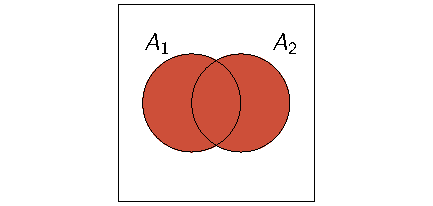
\includegraphics{Resources/Plots/Vereinigung-1} \end{center}
\normalsize
\end{frame}

\begin{frame}{Grundlegende Begriffe}
\phantomsection\label{grundlegende-begriffe-11}
\framesubtitle{Durchschnittsereignis}

\begin{itemize}
\tightlist
\item
  Ist der Schnitt zweier Ereignisse \(A_i\) und \(A_j\) nicht leer, gilt
  \(A_i\cap A_j=D\neq\emptyset\), so treten mit \(D\) auch die
  Ereignisse \(A_i\) und \(A_j\) ein.
\item
  \(D\) heißt daher \hil{Durchschnittsereignis}, das allgemein definiert
  ist als \(D=\bigcap_{j=1}^n A_j\). \(D\) tritt ein, wenn alle \(A_j\)
  eintreten.
\end{itemize}

\vspace{-0.5cm}

\footnotesize
\begin{center}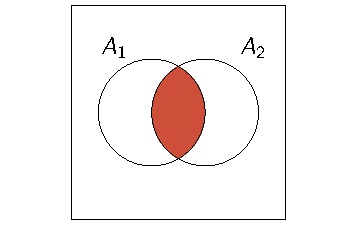
\includegraphics{Resources/Plots/Durchschnitt-1} \end{center}
\normalsize
\end{frame}

\begin{frame}{Grundlegende Begriffe}
\phantomsection\label{grundlegende-begriffe-12}
\framesubtitle{Komplementärereignis}

\begin{itemize}
\tightlist
\item
  Tritt \(A_i\) genau dann ein, wenn \(A_j\) nicht eintritt, so sind die
  beiden Ereignisse zueinander komplementär.
\item
  \(A_i\) heißt \hil{Komplementärereignis} oder kurz Komplement und
  lässt sich schreiben als \(A_i=\bar{A}_j\). Natürlich ist auch \(A_j\)
  Komplementärereignis zu \(A_i\): \(A_j = \bar{A}_i\).
\item
  Im Beispiel \ref{xmpl:potenz} ist das Ereignis \(A_2=\{1\}\) das
  Komplement zu \(A_7 =\{2,3\}:A_2=\bar{A}_7.\) Umgekehrt gilt auch
  \(A_7=\bar{A}_2\).
\item
  Für \(A\) und sein Komplement \(\bar{A}\) gelten
  \(A \cup \bar{A} = \Omega\) und \(A \cap \bar{A} = \emptyset\).
\end{itemize}

\footnotesize
\begin{center}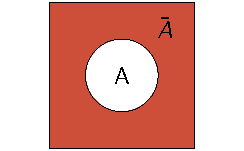
\includegraphics{Resources/Plots/Komplementaerereignis-1} \end{center}
\normalsize
\end{frame}

\begin{frame}{Grundlegende Begriffe}
\phantomsection\label{grundlegende-begriffe-13}
\framesubtitle{Teilereignisse und disjunkte Ereignisse}

\begin{itemize}
\tightlist
\item
  \(A_i\) und \(A_j\) heißen \hil{disjunkt}, wenn ihr Schnitt leer ist:
  \(A_i\cap A_j =\emptyset\).
\item
  Komplementäre Ereignisse sind daher immer auch disjunkt, die Umkehrung
  gilt aber nicht.
\item
  So sind im Beispiel \ref{xmpl:potenz} \(A_2=\{1\}\) und
  \(A_3 = \{2\}\) zwar disjunkt, aber nicht komplementär. Denn wenn
  \(A_3\) nicht eintritt, folgt nicht notwendigerweise das Eintreten von
  \(A_2\); es könnte auch \(A_4=\{3\}\) eintreten.
\end{itemize}

\footnotesize
\begin{center}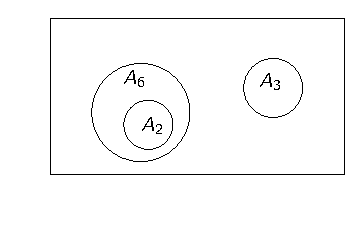
\includegraphics{Resources/Plots/Disjunkt-1} \end{center}
\normalsize
\end{frame}

\begin{frame}{Grundlegende Begriffe}
\phantomsection\label{grundlegende-begriffe-14}
\framesubtitle{Teilereignisse und disjunkte Ereignisse}

\begin{itemize}
\tightlist
\item
  \(A_i\) ist ein \hil{Teilereignis} von \(A_j\), wenn jeder Ausgang
  eines Zufallsvorgangs, der zu \(A_i\) gehört, auch in \(A_j\) liegt,
  \(A_j\) aber mindestens einen Ausgang \(\omega_j\) enthält, der nicht
  auch in \(A_i\) enthalten ist.
\item
  \(A_i\) ist eine \hil{echte Teilmenge} von \(A_j:\)
  \(A_i\subset A_j\).
\item
  In der Abbildung repräsentieren die Kreise die Ereignisse \(A_2\),
  \(A_3\) und \(A_6\) des Beispiels \ref{xmpl:potenz}.
\end{itemize}
\end{frame}

\begin{frame}{Grundlegende Begriffe}
\phantomsection\label{grundlegende-begriffe-15}
\framesubtitle{Differenzereignis}

\begin{itemize}
\tightlist
\item
  Das \hil{Differenzereignis} \(A_i\setminus A_j\) tritt dann ein, wenn
  der Ausgang des Zufallsvorgangs in \(A_i\), aber nicht in \(A_j\)
  liegt.
\item
  Man nennt \(A_i\setminus A_j\) auch das \hil{relative Komplement} zu
  \(A_j\) bezüglich \(A_i\). Alternativ kann man schreiben
  \(A_i\setminus A_j=A_i\cap\bar{A}_j\). Im Beispiel \ref{xmpl:potenz}
  folgt für \(A_6 = \{1,3\}\) und \(A_5 = \{1,2\}\) das
  Differenzereignis \(A_6\setminus A_5\) als
  \[A_6\setminus A_5 = A_6\cap\bar{A}_5 = \{1,3\}\cap\{3\}=\{3\}.\] Nur
  \(\omega_3=3\) führt dazu, dass \(A_6\setminus A_5\) eintritt. Das
  Beispiel zeigt, dass im Allgemeinen
  \(A_i\setminus A_j \neq A_j\setminus A_i\).
\end{itemize}

\vspace{-0.75em}

\footnotesize
\begin{center}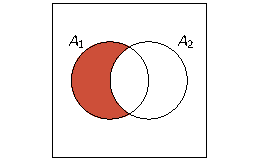
\includegraphics{Resources/Plots/Differenzmenge-1} \end{center}
\normalsize
\end{frame}

\begin{frame}{Grundlegende Begriffe}
\phantomsection\label{grundlegende-begriffe-16}
\framesubtitle{Ereignisse - QuizAcademy}

\QuizAcademy{Würfelwurf 1}\endQuizAcademy
\end{frame}

\begin{frame}[fragile]{Grundlegende Begriffe}
\phantomsection\label{grundlegende-begriffe-17}
\framesubtitle{Mengen in R}

\footnotesize

\begin{Shaded}
\begin{Highlighting}[]
\NormalTok{x }\OtherTok{\textless{}{-}} \FunctionTok{c}\NormalTok{(}\DecValTok{1}\NormalTok{,}\DecValTok{3}\NormalTok{,}\DecValTok{5}\NormalTok{)}
\NormalTok{y }\OtherTok{\textless{}{-}} \FunctionTok{c}\NormalTok{(}\DecValTok{2}\NormalTok{,}\DecValTok{3}\NormalTok{,}\DecValTok{6}\NormalTok{)}

\FunctionTok{union}\NormalTok{(x,y)}
\end{Highlighting}
\end{Shaded}

\begin{verbatim}
## [1] 1 3 5 2 6
\end{verbatim}

\begin{Shaded}
\begin{Highlighting}[]
\FunctionTok{intersect}\NormalTok{(x,y)}
\end{Highlighting}
\end{Shaded}

\begin{verbatim}
## [1] 3
\end{verbatim}

\begin{Shaded}
\begin{Highlighting}[]
\FunctionTok{setdiff}\NormalTok{(x,y)}
\end{Highlighting}
\end{Shaded}

\begin{verbatim}
## [1] 1 5
\end{verbatim}

\begin{Shaded}
\begin{Highlighting}[]
\FunctionTok{setdiff}\NormalTok{(y,x)}
\end{Highlighting}
\end{Shaded}

\begin{verbatim}
## [1] 2 6
\end{verbatim}

\begin{Shaded}
\begin{Highlighting}[]
\FunctionTok{setdiff}\NormalTok{(}\FunctionTok{union}\NormalTok{(x,y),y) }\CommentTok{\# Komplement von y, wenn Omega = union(x,y)}
\end{Highlighting}
\end{Shaded}

\begin{verbatim}
## [1] 1 5
\end{verbatim}

\normalsize
\end{frame}

\begin{frame}[fragile]{Grundlegende Begriffe}
\phantomsection\label{grundlegende-begriffe-18}
\framesubtitle{Mengen in R}

\scriptsize

\begin{Shaded}
\begin{Highlighting}[]
\NormalTok{rje}\SpecialCharTok{::}\FunctionTok{powerSet}\NormalTok{(x)}
\end{Highlighting}
\end{Shaded}

\begin{verbatim}
## [[1]]
## numeric(0)
## 
## [[2]]
## [1] 1
## 
## [[3]]
## [1] 3
## 
## [[4]]
## [1] 1 3
## 
## [[5]]
## [1] 5
## 
## [[6]]
## [1] 1 5
## 
## [[7]]
## [1] 3 5
## 
## [[8]]
## [1] 1 3 5
\end{verbatim}

\normalsize
\end{frame}

\begin{frame}{Grundlegende Begriffe}
\phantomsection\label{grundlegende-begriffe-19}
\framesubtitle{Ereignisse}

\exe[]Ein Würfel wird einmal gewürfelt. Es sind folgende Ereignisse
definiert: \begin{gather*}
A_1=\{1,2\},\; A_2=\{3,4\},\; A_3=\{2,4\},\; A_4=\{1,2,3,4\},\\ A_5=\{4\}, A_6=\{3,4,5,6\}, A_7=\{5,6\},\; A_8=\{1,2,4,5\},\\ A_9=\{2,3,6\},\; A_{10}=\{1,4,5\}.
\end{gather*}

Bestimmen Sie folgende Ereignisse und stellen Sie diese jeweils in einem
Venn-Diagramm grafisch dar!

\begin{center}
\begin{tabular}{lll}
\blue{(a)} $A_1\cup A_2$ & \blue{(b)} $A_2\cap A_3$ & \blue{(c)} $\bar{A}_1$\\
\blue{(d)} $A_1\cap A_2$ & \blue{(e)} $A_8\cap\bar{A}_9=A_8\setminus A_9$ & \blue{(f)} $A_5\subset A_4$
\end{tabular}
\end{center}

\endexe
\end{frame}

\begin{frame}{Grundlegende Begriffe}
\phantomsection\label{grundlegende-begriffe-20}
\framesubtitle{Ereignisse}

\begin{itemize}
\tightlist
\item
  Jedes zusammengesetzte Ereignis \(A\) kann in disjunkte Teilereignisse
  \(A_j\neq\emptyset\) so zerlegt werden, dass gilt:
  \(A=\bigcup^n_{j=1} A_j\). \(A\) ergibt sich jetzt als disjunkte
  Vereinigung.
\item
  In Beispiel \ref{xmpl:potenz} lässt sich \(A_8\) in \(A_2=\{1\}\) und
  \(A_7=\{2,3\}\), aber auch in \(A_2=\{1\}\), \(A_3=\{2\}\) und
  \(A_4=\{3\}\) zerlegen. Beim zweiten Fall wurde \(A_8\) in
  Elementarereignisse zerlegt.
\item
  Die Zerlegung von \(A\) in Elementarereignisse heißt
  \hil{kanonische Darstellung}: Jedes Ereignis ergibt sich eindeutig als
  Vereinigungsereignis von Elementarereignissen:
\end{itemize}

\[A=\bigcup^n_{j=1}\{\omega_j\}.\]
\end{frame}

\begin{frame}{Grundlegende Begriffe}
\phantomsection\label{grundlegende-begriffe-21}
\framesubtitle{Vollständiges Ereignissystem}

\begin{itemize}
\tightlist
\item
  Da auch \(\Omega\) zu den zusammengesetzten Ereignissen gehört, kann
  es auch in (Teil-)Ereignisse \(A_j\) zerlegt werden.
\item
  Die Menge \(\{A_1,\ldots,A_n\}\) bildet ein \hil{vollständiges
  System von Ereignissen}, wenn für diese Zerlegung gilt:
\end{itemize}

\begin{align*}
(1) \qquad & \Omega=A_1\cup\ldots\cup A_n=\bigcup^n_{j=1}A_j,\\
(2) \qquad & A_i\cap A_j=\emptyset\quad\text{für  $i\neq j$},\\
(3) \qquad & A_j\neq\emptyset\quad\text{für $j=1,\ldots,n$},
\end{align*}

\begin{itemize}
\tightlist
\item
  Ein vollständiges System wird auch \hil{vollständiges Ereignissystem}
  bzw. \hil{vollständige Zerlegung} genannt.
\end{itemize}
\end{frame}

\begin{frame}{Grundlegende Begriffe}
\phantomsection\label{grundlegende-begriffe-22}
\framesubtitle{Vollständiges Ereignissystem}

\footnotesize
\begin{center}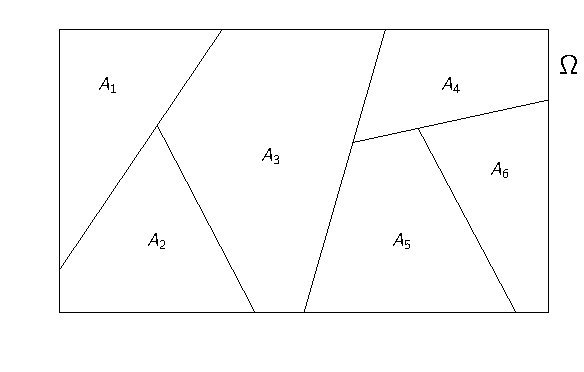
\includegraphics{Resources/Plots/unnamed-chunk-3-1} \end{center}
\normalsize
\end{frame}

\begin{frame}{Grundlegende Begriffe}
\phantomsection\label{grundlegende-begriffe-23}
\framesubtitle{Vollständiges Ereignissystem}

\exe

Ein Würfel wird einmal gewürfelt. Es sind folgende Ereignisse definiert:
\begin{gather*}
A_1=\{2,4,6\},\; A_2=\{1,3,5\},\; A_3=\{2\},\\
A_4=\{4,6\},\;A_5=\{1,3\}, A_6=\{5,6\}.
\end{gather*} Welche der folgenden Mengen bildet ein vollständiges
Ereignissystem?

\begin{enumerate}
[(a)]
\tightlist
\item
  \(F_1=\{A_1, A_2\}\)
\item
  \(F_2=\{A_1, A_5, A_6\}\)
\item
  \(F_3=\{A_3, A_4, A_5\}\)
\item
  \(F_4=\{A_2, A_3, A_4\}\)
\end{enumerate}

\endexe
\end{frame}

\begin{frame}{Der Wahrscheinlichkeitsbegriff}
\phantomsection\label{der-wahrscheinlichkeitsbegriff}
\begin{itemize}
\tightlist
\item
  Zufallsvorgänge zeichnen sich dadurch aus, dass ungewiss ist, welches
  ihrer möglichen Ereignisse eintritt.
\item
  Wahrscheinlichkeiten quantifizieren die Chance des Eintretens eines
  bestimmten Ereignisses und werden mit \(P\) symbolisiert.
\item
  Für ein Ereignis \(A\subset\Omega\) gibt \(P(A)\) jetzt die
  \hil{Wahrscheinlichkeit} für das Eintreten von \(A\) an.
\item
  \(P\) ist also eine Funktion, die Ereignissen reelle Zahlen zuordnet,
  welche wir als Wahrscheinlichkeit bezeichnen.
\end{itemize}
\end{frame}

\begin{frame}{Der Wahrscheinlichkeitsbegriff}
\phantomsection\label{der-wahrscheinlichkeitsbegriff-1}
\framesubtitle{Wahrscheinlichkeitfunktion und Kolmogoroff-Axiome}

\begin{itemize}
\tightlist
\item
  Die axiomatische Grundlage für Wahrscheinlichkeiten wurde von
  \hil{Kolmogoroff} entwickelt.
\item
  Auf der Basis dieser Axiomatik lässt sich die
  Wahrscheinlichkeitsfunktion wie folgt definieren:
\end{itemize}

\block{Kolmogoroff-Axiome}
\begin{itemize}\tightlist
\leftskip=12pt
\item[(K1)] $P(A)\geq 0$ für alle $A$,
\item[(K2)] $P(\Omega)=1$,
\item[(K3)] $P\left(\bigcup^\infty_{j=1} A_j\right) = P(A_1)+P(A_2)  +\ldots=\sum^\infty_{j=1} P(A_j)$ 
  \begin{itemize}\tightlist
  \leftskip=12pt
    \item[] für alle $A_i$ und $A_j$, die paarweise disjunkt sind: $A_i\cap A_j=\emptyset,$ $i\neq j$.
  \end{itemize}
\end{itemize}

\endblock
\end{frame}

\begin{frame}{Der Wahrscheinlichkeitsbegriff}
\phantomsection\label{der-wahrscheinlichkeitsbegriff-2}
\framesubtitle{Wahrscheinlichkeitfunktion und Kolmogoroff-Axiome}

\block{Kolmogoroff-Axiome}
\begin{itemize}\tightlist
\leftskip=8pt
\item[(K1)] \hil{Nichtnegativität}: Die Wahrscheinlichkeit $P$ eines Ereignisses $A$ ist stets nichtnegativ.
\item[(K2)] \hil{Normierung} der Wahrscheinlichkeit.
\item[(K3)] \hil{Volladdidivität}: Die Wahrscheinlichkeit für die Vereinigung paarweise disjunkter Ereignisse gleicht der Summe der Einzelwahrscheinlichkeiten.
\end{itemize}
\endblock

Jedes Ereignis \(A\subset\Omega\) wird somit durch \(P\) in das
geschlossene Intervall \([0,1]\subset\mathbb{R}\) abgebildet.
\end{frame}

\begin{frame}{Der Wahrscheinlichkeitsbegriff}
\phantomsection\label{der-wahrscheinlichkeitsbegriff-3}
\framesubtitle{Rechenregeln}

Aus diesen Axiomen lassen sich folgende Rechenregeln ableiten:

\block{Rechenregeln}
 \begin{itemize}\tightlist\leftskip=12pt
\item[(R1)] $P(A)+P(\bar{A})=1,$
\item[(R2)] $P(A)\leq P(B)$ für $A\subset B$,
\item[(R3)] $P(A_1\cup A_2\cup\ldots\cup A_n)=\sum^n_{j=1}\limits P(A_j)$ (für paarweise disjunkte Ereignisse),
\item[(R4)] $P(A\cup B)=P(A)+P(B)-P(A\cap B)$ (für paarweise nicht disjunkte Ereignisse).
 \end{itemize}
\endblock

Ihre Herleitung findet sich im Buch auf S.~23.
\end{frame}

\begin{frame}{Der Wahrscheinlichkeitsbegriff}
\phantomsection\label{der-wahrscheinlichkeitsbegriff-4}
\framesubtitle{Rechenregeln - Additionssatz}

\[P(A\cup B)=P(A)+P(B)-\textcolor[RGB]{205,79,57}{P(A\cap B)}\]

\footnotesize
\begin{center}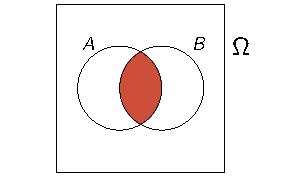
\includegraphics{Resources/Plots/unnamed-chunk-4-1} \end{center}
\normalsize

\begin{itemize}
\tightlist
\item
  \(A\) und \(B\) sind nicht disjunkt, da \(A\cap B \not=\emptyset\).
  \(A\cap B\) entspricht der roten Fläche.
\item
  \((A\cup B)\) würde mit \(P(A)+P(B)\) die Wahrscheinlichkeit für
  \(A\cap B\) doppelt erfassen; folglich muss \(P(A\cap B)\) subtrahiert
  werden.
\end{itemize}
\end{frame}

\begin{frame}{Der Wahrscheinlichkeitsbegriff}
\phantomsection\label{der-wahrscheinlichkeitsbegriff-5}
\framesubtitle{Rechenregeln}

\begin{itemize}
\tightlist
\item
  Der \hil{Additionssatz für disjunkte Ereignisse}
  \[P(A_1\cup A_2\cup\ldots\cup A_n)=\sum^n_{j=1}\limits P(A_j)\]
  liefert eine Vorschrift für die Wahrscheinlichkeit eines Ereignisses
  \(A=\{\omega_1,\omega_2,\ldots,\omega_n\}\) eines abzählbar
  unendlichen Stichprobenraumes \(\Omega\).
\item
  \hil{Elementarereignisse} \(\{\omega_j\},\) \(j=1,\ldots,n\) sind
  paarweise disjunkt.
\end{itemize}
\end{frame}

\begin{frame}{Der Wahrscheinlichkeitsbegriff}
\phantomsection\label{der-wahrscheinlichkeitsbegriff-6}
\framesubtitle{Rechenregeln}

\exe[]Es sind folgende Wahrscheinlichkeiten gegeben:
\[P(A)=0.4, P(B)=0.7, P(A\cap B)=0.25.\] Bestimmen Sie die
Wahrscheinlichkeiten
\[P(A\cup B),\;P(\bar{B}),\;P(A\cap \bar{B}),\;P(A\cup \bar{B})\]
\endexe Wir verwenden einen Punkt anstelle eines Kommas als
\hil{Dezimaltrennzeichen}, da dies der angloamerikanischen Schreibweise
der Programmiersprache \R entspricht.
\end{frame}

\begin{frame}{Der Wahrscheinlichkeitsbegriff}
\phantomsection\label{der-wahrscheinlichkeitsbegriff-7}
\framesubtitle{Rechenregeln}
\exe

Ein Würfel wird ein Mal gewürfelt. Wie groß ist die Wahrscheinlichkeit,

\begin{enumerate}
[a)]
\tightlist
\item
  eine 2 oder eine 3 zu würfeln?
\item
  eine 2, eine 3 oder eine 4 zu würfeln?
\item
  eine ungerade Zahl oder eine gerade Zahl zu würfeln?
\item
  eine Augenzahl kleiner als 4 oder eine gerade Augenzahl zu würfeln?
\item
  eine Augenzahl kleiner als 4 und eine gerade Augenzahl zu würfeln?
\end{enumerate}

\endexe
\end{frame}

\begin{frame}{Der Wahrscheinlichkeitsbegriff}
\phantomsection\label{der-wahrscheinlichkeitsbegriff-8}
\framesubtitle{Rechenregeln}
\exe

In einer Urne befinden sich 20 rote und 30 grüne Kugeln. 5 rote und 10
grüne Kugeln sind mit einer 1 beschriftet. Wie groß ist die
Wahrscheinlichkeit, dass

\begin{enumerate}
[a)]
\tightlist
\item
  eine gezogene Kugel rot oder mit einer 1 beschriftet ist?
\item
  eine gezogene Kugel nicht mit einer 1 beschriftet ist?
\item
  eine rote Kugel gezogen wird und diese nicht mit einer 1 beschriftet
  ist?
\item
  eine Kugel gezogen wird, die rot oder nicht mit einer 1 beschriftet
  ist?
\end{enumerate}

\endexe
\end{frame}

\begin{frame}{Der Wahrscheinlichkeitsbegriff}
\phantomsection\label{der-wahrscheinlichkeitsbegriff-9}
\framesubtitle{Wahrscheinlichkeitsinterpretation}

\begin{itemize}
\tightlist
\item
  Mit den \hil{Axiomen von Kolmogoroff} und den Regeln \blue{(R1)} bis
  \blue{(R4)} sind nur die allgemeinen Eigenschaften der
  Wahrscheinlichkeiten festgelegt, nicht jedoch welche Werte sie bei
  bestimmten Ereignissen annehmen.
\item
  Hierzu muss eine dem Zufallsvorgang adäquate
  \hil{Wahrscheinlichkeitsinterpretation} vorliegen.
\end{itemize}

Mit dem subjektiven und statistisch/frequentistischen
Wahrscheinlichkeitsbegriff befasst sich das Buch auf S.~25.
\end{frame}

\begin{frame}{Der Wahrscheinlichkeitsbegriff}
\phantomsection\label{der-wahrscheinlichkeitsbegriff-10}
\framesubtitle{Objektive Wahrscheinlichkeit}

\begin{center}
\begin{tikzpicture}
\node[box] (a) {Objektive\\Wahrscheinlichkeitsinterpretation};
\node[box ,below of=a, xshift=-2cm, yshift=-1cm] (b) {a priori};
\node[box, below of=a, xshift=2cm, yshift=-0.5cm] (c) {statistisch\\frequentistisch};
\node[box, below of=b, xshift=-1.5cm, yshift=-0.25cm] (d) {klassisch\\(Laplace)};
\node[box, below of=b, xshift=1.5cm] (e) {geometrisch};
\draw[arrow] (a) to (b);
\draw[arrow] (a) to (c);
\draw[arrow] (b) to (d);
\draw[arrow] (b) to (e);
\end{tikzpicture}
\end{center}
\end{frame}

\begin{frame}{Der Wahrscheinlichkeitsbegriff}
\phantomsection\label{der-wahrscheinlichkeitsbegriff-11}
\framesubtitle{Objektive Wahrscheinlichkeit}

\exe

Student Paul kommt jeden Morgen zwischen 8.00 und 8.30 Uhr an einer
Bushaltestelle an, an der zwei Buslinien halten: \begin{gather*}
\text{Linie A:}\quad 8.04, 8.14, 8.24 \\ 
\text{Linie B:}\quad 8.10, 8.20, 8.30.
\end{gather*} Wie groß ist die Wahrscheinlichkeit, dass er Linie A
nimmt? \endexe
\end{frame}

\begin{frame}{Der Wahrscheinlichkeitsbegriff}
\phantomsection\label{der-wahrscheinlichkeitsbegriff-12}
\framesubtitle{Objektive Wahrscheinlichkeit}

\begin{itemize}
\tightlist
\item
  \hil{a-priori}:

  \begin{itemize}
  \item
    \hil{Laplace- (bzw. klassische) Wahrscheinlichkeit}: Anwendung bei
    Zufallsvorgängen mit endlichem \(\Omega\) und deren
    Elementarereignisse die gleiche Eintrittswahrscheinlichkeit besitzen
    (\hil{Laplace-Experimente}).
  \item
    Laplace-Experimente können als die zufällige Entnahme aus einer
    endlichen Menge von Objekten charakterisiert werden. Wird mehrfach
    gezogen, muss zwischen \emph{Ziehen mit Zurücklegen} oder
    \emph{Ziehen ohne Zurücklegen} unterschieden werden.
  \end{itemize}
\end{itemize}
\end{frame}

\begin{frame}{Der Wahrscheinlichkeitsbegriff}
\phantomsection\label{der-wahrscheinlichkeitsbegriff-13}
\framesubtitle{Laplace-Wahrscheinlichkeit}

\block{Laplace-Wahrscheinlichkeit}

Die Wahrscheinlichkeit für ein Elementarereignis \(\{\omega_i\},\)
\(i=1,\ldots,m\) beträgt dann \(P(\{\omega_i\})=\frac{1}{m}\).\mps

\(P(A)\) erhält man als \[
  P(A)=\dfrac{\text{Anzahl der für $A$ günstigen Ausgänge}}{\text{Anzahl der möglichen Ausgänge}}.
  \] Die Anzahl der Elemente einer Menge \(M\) heißt \hil{Mächtigkeit}
\(|M|\). Die Laplace-Wahrscheinlichkeit ist dann
\[P(A)=\frac{|A|}{|\Omega|}.\] \endblock
\end{frame}

\begin{frame}{Der Wahrscheinlichkeitsbegriff}
\phantomsection\label{der-wahrscheinlichkeitsbegriff-14}
\framesubtitle{Laplace-Wahrscheinlichkeit - QuizAcademy}

\QuizAcademy{Würfelwurf 2}\endQuizAcademy
\end{frame}

\begin{frame}{Der Wahrscheinlichkeitsbegriff}
\phantomsection\label{der-wahrscheinlichkeitsbegriff-15}
\framesubtitle{Laplace-Wahrscheinlichkeit}
\exe[Laplace-Experimente]

\begin{enumerate}
[(a)]
\tightlist
\item
  In einer Urne befinden sich 20 Kugeln, von denen 8 rot sind. Berechnen
  Sie die Wahrscheinlichkeit eine rote Kugel bei einer zufälligen
  Entnahme zu erhalten.
\item
  Wie groß ist die Wahrscheinlichkeit, nach Ziehen einer roten Kugel
  ohne Zurücklegen im zweiten Zug erneut eine rote Kugel zu ziehen?
\item
  Ein \hil{Laplace-Würfel} (idealer Würfel) wird geworfen. Berechnen Sie
  die Wahrscheinlichkeit, dass eine Augenzahl größer als 2 oben liegt.
\end{enumerate}

\endexe
\end{frame}

\begin{frame}{Der Wahrscheinlichkeitsbegriff}
\phantomsection\label{der-wahrscheinlichkeitsbegriff-16}
\framesubtitle{Laplace-Wahrscheinlichkeit}

\exe[]Ein Laplace-Würfel wird einmal geworfen. Wie groß ist die
Wahrscheinlichkeit, dass eine Augenzahl kleiner 3 fällt? \endexe
\exe[]Eine Laplace-Münze und ein Laplace-Würfel werden gemeinsam
geworfen. Wie groß ist die Wahrscheinlichkeit, dass Kopf und eine
Augenzahl größer als 4 fällt? \endexe
\end{frame}

\begin{frame}{Bedingte Wahrscheinlichkeit}
\phantomsection\label{bedingte-wahrscheinlichkeit}
\framesubtitle{Änderung des Stichprobenraums}
\vspace{0.5cm}

\begin{itemize}
\tightlist
\item
  Die Berechnung von Wahrscheinlichkeiten erfolgt bislang unter Bezug
  auf den ganzen Stichprobenraum \(\Omega\).
\item
  Es lassen sich aber auch dann Wahrscheinlichkeiten für \(A\)
  berechnen, wenn nicht ganz \(\Omega\), sondern nur noch ein Teil \(B\)
  davon relevant ist. Die Abbildung verdeutlicht die Veränderung des
  Bezugssystems.
\end{itemize}

\vspace{-.5cm}

\footnotesize
\begin{center}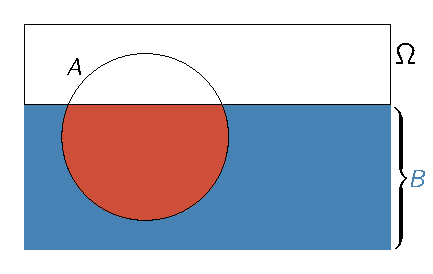
\includegraphics{Resources/Plots/BedingteWkeit-1} \end{center}
\normalsize
\end{frame}

\begin{frame}{Bedingte Wahrscheinlichkeit}
\phantomsection\label{bedingte-wahrscheinlichkeit-1}
\framesubtitle{Änderung des Stichprobenraums}

\begin{itemize}
\tightlist
\item
  Der Kreis entspricht \(A\), das untere Rechteck \(B\) und das rote
  Kreissegment \(A\cap B\).
\item
  \(P(A)\), \(P(B)\) und \(P(A\cap B)\) sind die Wahrscheinlichkeiten
  für \(A\), \(B\) und \(A\cap B\), wenn \(\Omega\) zugrunde liegt.
\item
  Es kann aber auch die Wahrscheinlichkeit für \(A\) unter der Bedingung
  berechnet werden, dass nur noch die Ausgänge in \(B\) relevant sind.
\item
  Diese \hil{bedingte Wahrscheinlichkeit} wird mit \(P(A|B)\)
  bezeichnet.
\item
  In der Abbildung ist \(P(A)\) das Verhältnis der Kreisfläche zur
  Fläche des Rechtecks \(\Omega\); die bedingte Wahrscheinlichkeit
  \(P(A|B)\) jedoch das Verhältnis der roten Fläche zur Fläche des
  Rechtecks \(B\).
\end{itemize}
\end{frame}

\begin{frame}{Bedingte Wahrscheinlichkeit}
\phantomsection\label{bedingte-wahrscheinlichkeit-2}
\framesubtitle{Formel}

\begin{block}{Bedingte Wahrscheinlichkeit}
 Es seien $A$, $B\subset\Omega$ Ereignisse
 und %$(\Omega, A, P)$ der Wahrscheinlichkeitsraum,
 $P(B) > 0$. Für die \hil{bedingte Wahrscheinlichkeit} $P(A|B)$ gilt \[ P(A|B) = \frac{P(A\cap B)}{P(B)}. \]
\end{block}
\end{frame}

\begin{frame}{Bedingte Wahrscheinlichkeit}
\phantomsection\label{bedingte-wahrscheinlichkeit-3}
\framesubtitle{Beispiele}

\xmpl[Idealer Würfel]Ein idealer Würfel wird geworfen. Also sind
\(\Omega =\{1,2,\ldots,6\}\) und \(P(\{\omega_i\}) = 1/6\) für
\(i=1,\ldots,6\). \medskip

\(A\) ist das Ereignis, eine \emph{1} zu würfeln; \(B\) das Ereignis
einer ungeraden Augenzahl. \(A\cap B\) tritt bei einer \emph{1} ein. Die
Wahrscheinlichkeiten betragen \(P(A) = 1/6,\) \(P(B) = 1/2\) und
\(P(A\cap B) = 1/6\). \medskip

Was ist nun die Wahrscheinlichkeit einer \emph{1} unter der Bedingung,
dass eine ungerade Augenzahl eintritt? Der durch die Bedingung gegebene
Stichprobenraum lautet \(B = \{1,3,5\}\), also gilt \(P(A|B)=1/3.\)
\medskip

Denselben Wert erhält man nach der eingeführten Definition:
\[ P(A|B) = \frac{P(A\cap B)}{P(B)} = \frac{\frac{1}{6}}{\frac{1}{2}}=\frac{1}{3}.\]
\endxmpl
\end{frame}

\begin{frame}{Bedingte Wahrscheinlichkeit}
\phantomsection\label{bedingte-wahrscheinlichkeit-4}
\framesubtitle{Aufgaben}
\exe

Nach der achtmaligen Durchführung des Zufallsexperiments
\emph{zweimaliges Werfen einer Münze} erhält man folgendes Resultat:

\begin{center}
\begin{tabular}{l|cccccccc}
Versuch & 1 & 2 & 3 & 4 & 5 & 6 & 7 & 8\\ \hline
1. Wurf & K & Z & Z & Z & K & Z & Z & K\\
2. Wurf & Z & Z & K & K & K & Z & K & Z
\end{tabular}
\end{center}

Ereignis \(A\): K beim 1. Wurf,\quad Ereignis \(B\): K beim 2. Wurf

Berechnen Sie folgende Wahrscheinlichkeiten:

\begin{center}
\begin{tabular}{lll}
\blue{(a)} $P(A)$   & \blue{(b)} $P(B)$   & \blue{(c)} $P(A\cap B)$\\
\blue{(d)} $P(A|B)$ & \blue{(e)} $P(B|A)$ & \\
\end{tabular}
\end{center}
\endexe
\end{frame}

\begin{frame}{Bedingte Wahrscheinlichkeit}
\phantomsection\label{bedingte-wahrscheinlichkeit-5}
\framesubtitle{Aufgaben}
\exe

In einem Dorf leben 1000 Personen. Es ist bekannt, dass 600 Einwohner
nach Mallorca in den Urlaub fahren und dass 500 Einwohner die
Bild--Zeitung lesen. Zusätzlich weiß man, dass von den 600
Mallorca--Urlaubern 400 die Bild lesen. Wie groß ist die
Wahrscheinlichkeit, dass

\begin{enumerate}
[(a)]
\tightlist
\item
  eine Person Mallorca--Urlauber ist,
\item
  eine Person Bild--Zeitung--Leser ist,
\item
  eine Person Mallorca--Urlauber und Bild--Zeitung--Leser ist,
\item
  wenn ein Einwohner Bild--Zeitung liest, dieser auch ein
  Mallorca--Urlauber ist,
\item
  wenn ein Einwohner Mallorca--Urlauber ist, dieser auch Bild--Zeitung
  liest?
\end{enumerate}

\endexe
\end{frame}

\begin{frame}{Bedingte Wahrscheinlichkeit}
\phantomsection\label{bedingte-wahrscheinlichkeit-6}
\framesubtitle{Paarweise stochastische Unabhängigkeit}

\begin{itemize}
\tightlist
\item
  \(P(A|B)\) lässt sich als die Wahrscheinlichkeit von \(A\) unter der
  zusätzlichen Information interpretieren, dass \(B\) bereits
  eingetreten ist.
\item
  Übt diese Information keinen Einfluss auf die Wahrscheinlichkeit von
  \(A\) aus, gilt \(P(A|B)=P(A)\).
\item
  \(A\) ist dann \hil{unabhängig} von \(B\).
\item
  Dann ist aber auch \(B\) unabhängig von \(A\), wie folgende Umformung
  zeigt: \begin{align*}
  P(B|A) & = \frac{P(A\cap B)}{P(A)}=\frac{P(A|B)P(B)}{P(A)} \\
   & = \frac{P(A)P(B)}{P(A)}=P(B)\;\;\; (\text{wegen }P(A|B)=P(A)).
  \end{align*}
\end{itemize}
\end{frame}




\end{document}